\documentclass[12pt]{article}
\usepackage{inputenc}
\usepackage{fancyhdr}
\usepackage{graphicx}
\pagestyle{fancy}
\rhead{\it{Navigator For Visually Impaired Person}}
\chead{}
\lhead{}

\begin{document}
	\begin{center}
		\LARGE{\underline{SYNOPSIS}}\\
	\end{center}
	
	\begin{tabbing}
		\hspace*{2 in}    \= :Mr. S. Wategavkar    \kill
		% \> for next tab, \\ for new line...
		\textbf{1.Name of the College} \> : Bharati  Vidyapeeth College of Engineering Navi \\
		\textbf{} \> \hspace{0.18cm} Mumbai \\
		\\
		\textbf{2.Name of the Course}\>  : B.E. (Electronics \& Telecommunication) \textbf{Div}: A \\
		\\
		\textbf{3.Name of the Students}\>  : 1) Nikhil Kanitkar (23)\\
		\textbf{}\>: 2) Dewoo Kudtarkar (27)\\
		\textbf{}\>: 3) Mandar Naik (40)\\
		\textbf{}\>: 4) Pranit Patil (48)\\
		\\
		
		\textbf{4.Name of the Guide}\>  : Prof. S.S. Patil                   \\
		\textbf{}\> \hspace{0.18cm} Department of Electronics \& Telecommunication \\ \textbf{} \> \hspace{0.18cm}  Engineering, \\
		\textbf{}\>\hspace{0.18cm} Bharati  Vidyapeeth College of Engineering Navi  \\
		\textbf{} \>\hspace{0.18cm}  Mumbai \\
		\\
		\textbf{5.Title of Project}\>  :  Navigator For Visually Impaired Person                \\
		\\
		\textbf{6.Problem Definition}\>  : Visually impaired individuals will face many difficulties\\ \hspace{5.4cm} and one of the common difficulties is when they are\\ \hspace{5.4cm} involved  in  self-navigating in an environment that is\\ \hspace{5.4cm} strange for them.  Physical movement is one of the biggest \\ \hspace{5.4cm} challenges for them.  Besides that, while they travel around \\ \hspace{5.4cm} or walk in a crowded corridor, it may pose great difficulty. \\ \hspace{5.4cm} One of the existing  problems for visually impaired individuals \\ \hspace{5.4cm} to travel in a passage is that they cannot detect whether \\ \hspace{5.4cm} they need to turn left or right when reached to the end \\ \hspace{5.4cm} of the corridor by using only a walking stick.            \\
		
		\\
		\textbf{7.Introduction}\>  :  Globally, At least 2.2 billion people have near or distant\\ \hspace{5.4cm} vision impairment. In at least 1 billion – or nearly half\\ \hspace{5.4cm} of these cases, vision impairment could have been prevented\\ \hspace{5.4cm} or has yet to be addressed. In another way creating a fusion\\ \hspace{5.4cm} of sensing technology and voice-based guidance system,\\ \hspace{5.4cm} products can be developed which could give better results\\ \hspace{5.4cm}  than individual technology.                \\
		
		Advantages: \hspace{2.9cm} 1) Both indoor and outdoor navigation are possible with the\\ \hspace{5.8cm} device \\ \hspace{5.5cm}2) Detects obstacles and notifies the blind person through\\ \hspace{5.9cm} vibration and speech production \\ 
		
		\\
		
		
		Applications: \hspace{2.7cm} 1) It can be used for providing a set of useful features :-\\ \hspace{5.8cm}  light detection, color detection, object recognition,\\ \hspace{5.8cm} and banknote recognition
		
		\\
		
		\\
		
		
		
		
		
		
		\textbf{8.Relevance/Motivation}\>  : The major motivation behind our project is to maintain a\\ \hspace{5.4cm} good functional system for visually impaired individuals.\\ \hspace{5.4cm}  This system can help visually impaired individuals to avoid\\ \hspace{5.4cm} the obstacles such as people and animals in outdoor places\\ \hspace{5.4cm} same with them, and it also can provide the distance of the\\ \hspace{5.4cm} obstacles in front of them.                  \\
		\\
		
		
		\textbf{9.Literature Review: }\>                 \\
		\\
		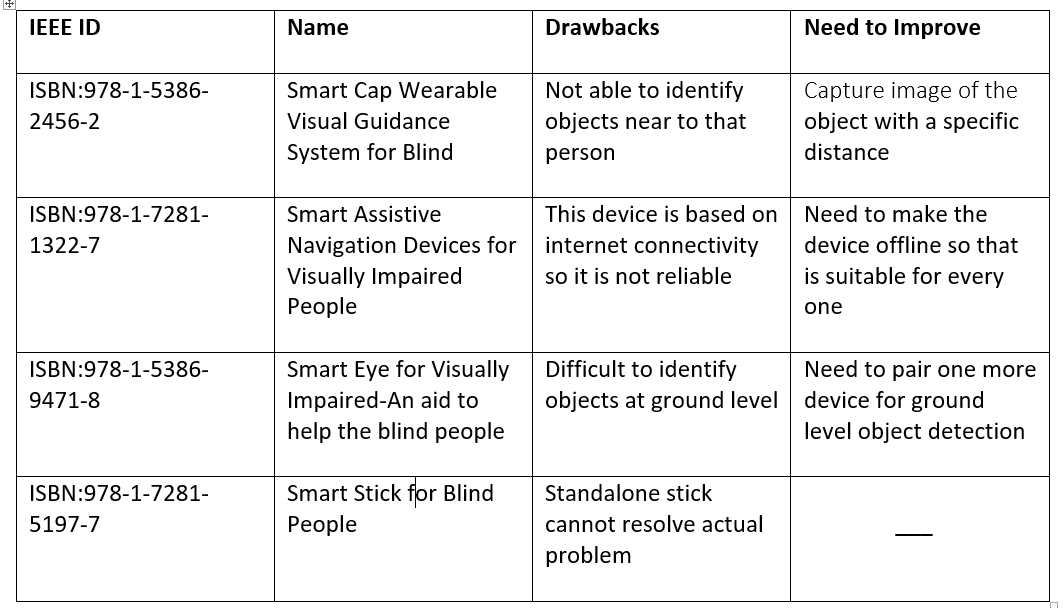
\includegraphics[width=16cm]{../Screenshot (10).png}
		
		\\
		\\
		
		
		
		\textbf{10.Proposed Work: }\>  \\    
		
		
		
		
		
		\hspace{1in} \textbf{a) Planning:}\>  \\ \hspace{5.4cm} The main objective of our present work is to provide a\\ \hspace{5.4cm} reliable, cost-effective, low-power solution for blind people\\ \hspace{5.4cm} which would help them to move almost like any other\\ \hspace{5.4cm} normal pedestrian. The cost of this system makes it \\ \hspace{5.4cm} affordable for the majority of society which in turn is an\\ \hspace{5.4cm} effective device for them to spend on, just for once,\\ \hspace{5.4cm} and assures wonderful travel guide for them. \\
		
		\\
		
		
		\hspace{1in} \textbf{b) Methodology \& Tools:}\> \\ \hspace{5.4cm} 1) The camera unit is responsible for capturing objects while
		\\ \hspace{5.6cm}the sensor unit provides the distance of object from unit.
		\\ \hspace{5.4cm} 2) The processing unit plays an important role in detecting and\\ \hspace{5.4cm} identifying objects (image processing) ,it also receives data from\\ \hspace{5.4cm} ultrasonic sensor then instruct the user about object identified\\ \hspace{5.4cm} and distance it is located at (So the user can navigate\\ \hspace{5.4cm} accordingly).
		
		\\
		
		\\
		
		
		\hspace{1in} \textbf{c) Facilities Available \& Requirement:}\>: \\ \hspace{5.4cm} Thonny IDE, Arduino IDE \\
		
		
		
		\\
		\hspace{1in} \textbf{d) REFERENCES:}\>
		\\ \hspace{5.4cm}1) ISBN:978-1-5386-2456-2 "Smart Cap  Wearable\\ \hspace{5.6cm} Visual Guidance System For Blind"
		\\ \hspace{5.4cm}2) ISBN:978-1-7281-1322-7 "Smart Assistive Navigation\\ \hspace{5.6cm} Devices for Visually Impaired People"
		\\ \hspace{5.4cm}3) ISBN:978-1-5386-9471-8 "Smart Eye for Visually Impaired\\ \hspace{5.6cm} -An aid to help the blind"
		\\
		
		
		\\
		
		
		
		\textbf{11.Approximate Expenditure:}\> \hspace{2cm} Rs.\hspace{0.2cm}7000-8000/-       \\
		
		\\
		\\
		\\
		
		
		
		Place: Navi Mumbai\\
		
		Date:\hspace{0.1cm} 08/10/2022
	\end{tabbing}
	
\end{document}